%%%%%%%%%%%%%%%%%%%%%%%%%%%%%%%%%%%%%%%%%
% Beamer Presentation
% LaTeX Template
% Version 1.0 (10/11/12)
%
% This template has been downloaded from:
% http://www.LaTeXTemplates.com
%
% License:
% CC BY-NC-SA 3.0 (http://creativecommons.org/licenses/by-nc-sa/3.0/)
%
%%%%%%%%%%%%%%%%%%%%%%%%%%%%%%%%%%%%%%%%%

%----------------------------------------------------------------------------------------
%	PACKAGES AND THEMES
%----------------------------------------------------------------------------------------

\documentclass[]{beamer}

\mode<presentation> {

% The Beamer class comes with a number of default slide themes
% which change the colors and layouts of slides. Below this is a list
% of all the themes, uncomment each in turn to see what they look like.

%\usetheme{metropolis}
%\usetheme{default}
%\usetheme{AnnArbor}
%\usetheme{Antibes}
%\usetheme{Bergen}
%\usetheme{Berkeley}
%\usetheme{Berlin}
%\usetheme{Boadilla}
%\usetheme{CambridgeUS}
%\usetheme{Copenhagen}
%\usetheme{Darmstadt}
%\usetheme{Dresden}
%\usetheme{Frankfurt}
%\usetheme{Goettingen}
%\usetheme{Hannover}
%\usetheme{Ilmenau}
%\usetheme{JuanLesPins}
%\usetheme{Luebeck}
%\usetheme{Madrid}
%\usetheme{Malmoe}
%\usetheme{Marburg}
%\usetheme{Montpellier}
%\usetheme{PaloAlto}
%\usetheme{Pittsburgh}
%\usetheme{Rochester}
%\usetheme{Singapore}
%\usetheme{Szeged}
%\usetheme{Warsaw}

% As well as themes, the Beamer class has a number of color themes
% for any slide theme. Uncomment each of these in turn to see how it
% changes the colors of your current slide theme.

%\usecolortheme{albatross}
%\usecolortheme{beaver}
%\usecolortheme{beetle}
%\usecolortheme{crane}
%\usecolortheme{dolphin}
%\usecolortheme{dove}
%\usecolortheme{fly}
%\usecolortheme{lily}
%\usecolortheme{orchid}
%\usecolortheme{rose}
%\usecolortheme{seagull}
%\usecolortheme{seahorse}
%\usecolortheme{whale}
%\usecolortheme{wolverine}

%\setbeamertemplate{footline} % To remove the footer line in all slides uncomment this line
%\setbeamertemplate{footline}[page number] % To replace the footer line in all slides with a simple slide count uncomment this line

%\setbeamertemplate{navigation symbols}{} % To remove the navigation symbols from the bottom of all slides uncomment this line
}

\usepackage{graphicx} % Allows including images
\usepackage{booktabs} % Allows the use of \toprule, \midrule and \bottomrule in tables
\usepackage[font=small,labelfont=bf]{caption}
\usepackage{tikz}
\usetikzlibrary{positioning}
\usepackage{booktabs}
\usepackage{siunitx}
\usepackage{float}
\usepackage{changepage}
\usepackage{mathtools}
\usepackage{amsmath}
\usepackage{bbm}
\usepackage{appendixnumberbeamer}
\usepackage{amssymb,amsmath}
\usetheme{cousteau}
\AtBeginSection[]
{
  \begin{frame}{Table of Contents}
    \tableofcontents[currentsection]
  \end{frame}
}

%----------------------------------------------------------------------------------------
%	TITLE PAGE
%----------------------------------------------------------------------------------------

\title{Gov 51 Section: Week 1} 

\subtitle{Conceptual Causality, DiD, IV}

\author[Cha]
{Jeremiah Cha} 
\institute
{
Harvard University
}
\date{} 

\begin{document}

\frame{\titlepage} 

\section{Introduction/Logistics}

\begin{frame}{Introduction}

\begin{itemize}
	\item G4 in the Government Department
	\item Congress, Racial Representation in Local Politics
	\item UC San Diego
	\item Pew Research Center
	\item Los Angeles
\end{itemize}

\end{frame}

\begin{frame}{Section Goals}
	\begin{itemize}
	\item Reinforce a solid foundation to engage with causal inference methodologies
	\item Develop a familiarity with machine learning in social science
	\item Understand methodological approaches in leading social science journals
	\item Work collaboratively on quantitative social science
\end{itemize}

\end{frame}

\begin{frame}{Section Syllabus}
	\begin{itemize}
		\item Full section syllabus can be found on Gov 51 course site 
		\item Office hours: Tuesday 10:00 AM - 12:00 PM (appointment basis) in CGIS Knafel Cafe
		\item Course Assistant Office Hours
		\begin{itemize}
			\item James Jolin: Wednesday 12:00 PM - 1:00 PM \& Thursday 1:30 PM - 2:30 PM (First 20 open, Last 40 appointment basis)
			\item Jack Wyss: Wednesday 7:00 PM - 9:00 PM
		\end{itemize}
	\end{itemize}
\end{frame}

\begin{frame}{Grading}
	\begin{itemize}
		\item Attendance is worth 20\% of your grade! This includes section. 
		\item Expectation in section is that you come prepared - much of what is covered will be extensions of your reading assignments and implementation! 
		\item While participation is not required, disrupting your classmates will impact your grade. 
		\item Alternative section attendance is fine - just email me AND James
	\end{itemize}
\end{frame}

\begin{frame}{Other Course Logistics}
	\begin{itemize}
		\item Gradescope set-up incoming - hold tight 
		\item Required math question 
		\item Base v.s. tidyverse 
		\item Laptops are required for both lecture and section 
		\item \pause Questions?
	\end{itemize}	
\end{frame}

\section{Causation and Correlation}

\begin{frame}{Causal Inference: A Crash Course}

\begin{itemize}
	\item Causal inference is the study of \textbf{causal} questions
	\begin{itemize}
		\item \pause Does an electoral challenge increase legislative productivity? 
		\item \pause Do protests lead to lasting institutional changes? 
	\end{itemize}
	\item Causal questions specifically revolve around unobserved outcomes
	\begin{itemize}
		\item Only one observed treatment outcome!
	\end{itemize}
	\item This is known as the \textbf{Fundamental Problem of Causal Inference}
\end{itemize}
	
\end{frame}

\begin{frame}{What Now?}
	\begin{itemize}
		\item Since we do not directly observe the counterfactual, how do we identify and estimate causal effects? 
		\item \pause Assumptions, assumptions, assumptions
		\item \pause But before that, let's introduce some notation to ground us 
	\end{itemize}
\end{frame}

\begin{frame}{Notation}
	\begin{itemize}
		\item $Y_i(T_i)$ where $Y_i$ refers to observation $i$'s outcome and $T_i$ refers to their treatment status 
		\item $Y_i(1)$: outcome that observation $i$ would have if treated.
		\item $Y_i(0)$: outcome that observation $i$ would have if untreated. 
		\item $E[X]$ is the \textbf{expectation or average} of random variable $X$
		\item For example, the $E[X]$, where $X$ is age, could be 20 for this class
	\end{itemize}
\end{frame}

\begin{frame}{Dataset Visualization}

\begin{table}[]
\begin{tabular}{lllllll}
\hline
\multicolumn{1}{|l}{Voters} & Age   & Gender & Canvassed & \multicolumn{2}{c}{Turnout} & \multicolumn{1}{l|}{Causal Effect}     \\
\multicolumn{1}{|l}{i}      & $X_1$ & $X_2$  & $T_i$     & $Y_i(1)$     & $Y_i(0)$     & \multicolumn{1}{l|}{$Y_i(1) - Y_i(0)$} \\ \hline
1                           & 19    & M      & 1         & 0            & ???          &  ???                                      \\
2                           & 56    & F      & 0         & ???          & 1            &  ???                                   \\
3                           & 89    & F      & 0         & ???          & 0            &  ???                                     
\end{tabular}
\end{table}
\end{frame}

\begin{frame}{Assumptions to Start}
	\begin{itemize}
		\item Given that we are unable to know the counterfactual for any given person, we employ the \textbf{Average Treatment Effect} as a measure of a causal effect oftentimes
		\item Asserting that the average effect = causal effect requires assumptions 
		\begin{enumerate}
			\item Non-interference among units 
			\item Only a single version of each treatment level (i.e. consistency)
		\end{enumerate}
		\item Together, these form the Stable Unit Treatment Value Assumption (SUTVA)
		\item These are just to start - there will be many more assumptions for other measures of causal effects
	\end{itemize}
\end{frame}

\begin{frame}
	Questions?
\end{frame}

\begin{frame}{Estimation v.s. Identification}
	\begin{itemize}
		\item Core distinction between identification and estimation (Blackwell 2013)
		\item Identification refers to the assumptions necessary to claim a causal effect
		\begin{itemize}
		\item IMPORTANT: "Identification tells us what to estimate, not how" 
		\end{itemize}
		\item Estimation is a statistical exercise that answers the how 
		\item We start with identification when we discuss instrumental variables, for example 
		\item \textbf{Estimand}: quantity we want to estimate
		\item \textbf{Estimator}: the method by which we measure the estimand 
	\end{itemize}
\end{frame}

\section{Difference-in-Difference}

\begin{frame}{Review}
	\begin{itemize}
		\item As in lecture, difference-in-difference allows us to ``infer what would have happened to the treatment group without treatment''
		\item What assumptions are necessary for identification? 
	\end{itemize}
	\centering
	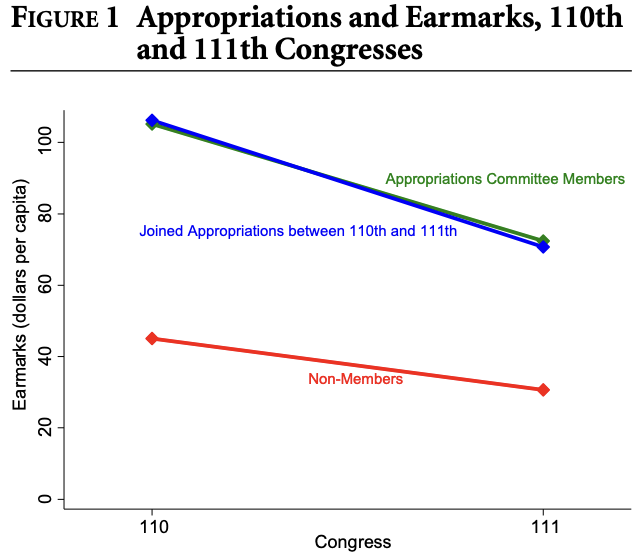
\includegraphics[scale=.5]{slideinputs/berryfowler.png}
\end{frame}

\begin{frame}{DiD Assumptions}

	\begin{itemize}
		\item \textbf{Parallel trends}: ``treated and control groups will share the same difference IF the treated were not to be treated at t = 1''
		\item You can do a difference-in-difference analysis without parallel trends (e.g. just simple algebra subtracting means) - your estimand will not be identified, so you cannot make causal interpretations 
		\item Difference-in-difference is a powerful tool in causal inference - they refer to a broad class of estimators that are hotly contested right now 
		\begin{itemize}
			\item Refinements include: DiDiD, moving treatments, controls in semi-parametric estimation, etc.
		\end{itemize}
	\end{itemize}
	
\end{frame}

\section{Instrumental Variables}

\begin{frame}{Why IV?}

	\begin{itemize}
		\item Explanatory variables are oftentimes correlated with our errors (endogeneity) 
		\item OLS and controls are \textbf{insufficient} to account for this bias 
		\item Example: conflict and economic growth, the efficacy of canvassing/mailers, the effect of TV consumption on political attitudes 
		\item Another way of framing? Confounders 
	\end{itemize}
	
\end{frame}

\begin{frame}{IV Assumptions}

	\begin{itemize}
		\item For IV to be identified, the instrumental variable must: 
	\begin{enumerate}
		\item Be assigned as-if random
		\item Affect treatment assignment
		\item Only affect outcome through treatment (Exclusion restriction)
		\item Not induce defiance (Monotonicity) 
	\end{enumerate}
		\item If these assumptions are met, our instrumental variable allow us to produce \textbf{consistent} estimate of the local Average Treatment Effect (LATE)
		\item The LATE is an estimate for only compliers - why? 
	\end{itemize}
\end{frame}

\begin{frame}{Assumptions Strike Back}
	
	\begin{itemize}
		\item The LATE is an estimate for only compliers - why? 
		\begin{itemize}
			\item The exclusion restriction means that always and never takers (e.g. no matter rain, economic downturn/no economic downturn) have the same treatment every time 
			\item If treatment is static, outcomes are \textbf{consistent}
			\item Monotonocity 
			\item Questions about its usefulness as our estimates are of an unknowable population 
		\end{itemize}
		\item Now that we've identified, how do we estimate? 
	\end{itemize}
\end{frame}

\begin{frame}{Estimator Example}

	\begin{itemize}
		\item A bunch of estimators exist for estimating the LATE - popular ones include the Wald or Two Stage Least Square (TSLS) estimators 
		\item Logic of TSLS 
		\begin{enumerate}
			\item Regress our treatment ($T_i$) on the instrument ($Z_i$)
			\item Regress our outcome ($Y_i$) on the fitted values of ($\widehat T_i$) we generated in the previous stage
		\end{enumerate}
		\item Important to note that we are \textbf{estimating} the LATE - because the proportions of compliers and always/never takers is unknown, we cannot estimate a true Average Treatment Effect (ATE) 
		\item In essence, using the variation caused by our instrument to address omitted variable bias
	\end{itemize}	
\end{frame}

\begin{frame}{Live Coding}

	
\end{frame}

\begin{frame}{Wrap-up}
	\begin{itemize}
		\item Causal inference assumptions 
		\item DiD as a powerful tool and simple implementation 
		\item Introduction to IV 
		\item If you need to change section, have questions, chat with me!
	\end{itemize}
\end{frame}
\end{document}